\textbf{Revised \today , at \currenttime}

\section{Introduction}

As a topic that is so important to life on Earth, biological light-harvesting systems have been a topic of interest for a long time ~\cite{Blankenship2002}.   Ever since the discovery of long-lived oscillations ($\approx$600 fs) in cross peaks of the two-dimensional electronic spectrum of the Fenna-Matthews-Olsen complex~\cite{FMO1}, interest surged because the observed oscillations could mean that photosynthetic chlorophylls were keeping a stable superposition of electronic-excited-states for much longer than a chaotic biological environment should be able to allow ~\cite{FMO2,Lambert2012}.

Because the ability to keep an electronic superposition (coherence) for a long amount of time has positive consequences for energy transfer rates and efficiencies~\cite{FMO1}, biological protection against electronic decoherence would be a profoundly interesting result of natural selection--one that we might hope to emulate.  Further research even suggested that there is an optimal point for energy transfer efficiency between perfect coherence and immediate dephasing that nature seemed to have found~\cite{energyTransfer} in the electronic dephasing rate of the Fenna-Matthews-Olsen complex and other photosynthetic complexes that were soon after discovered to have similar cross-peak oscillations ~\cite{Panitchayangkoon2011,Fidler2013,Collini2010}.  There is also great interest in being able to mimic these evolution-tuned efficiencies for artificial designs ~\cite{Creatore2013}.

Electronic coherence is not, however, the only process which contributes to the signal in an off-diagonal peak of a two-dimensional electronic spectrum; the vibrational motion of a molecule (also called vibrational coherences because multiple energy states are needed to produce motion) also contributes to the movement of cross peaks.  While much useful work has been done to pinpoint the  unique signatures of electronic coherence and the unique signatures of vibrational coherence in a two-dimensional electronic spectroscopy experiment ~\cite{FMO2,mech2,mech3,mech1,mech4}, a completely unambiguous experimental tool for the diagnosis of electronic coherences is still needed.

The desired experiment would give an concrete yes or no answer (called a witness in the language of quantum information~\cite{Chuang2005}) to the question of whether a system exhibits long-lived electronic superpositions.  In 2012, Yuen-Zhou et. al.~\cite{witness} developed such a witness using only a one dimensional pump-probe spectrum in the impulsive limit.  They showed that there are only oscillations in a pump probe spectrum when the pump and probe beams are impulsive, in the case where there is an electronic coherence present.  Otherwise there will be no oscillations present.


The effects of pulse widths on pump-probe spectroscopy had been studied previously~\cite{pulseWidth} but the proposed witness uniquely suggested using pulse width as an independent variable in an experiment, which should be feasible given developments in two-dimensional spectroscopy using pulse-shaping devices~\cite{pulse1,pulse2}.

Johnson et. al.  ~\cite{allanWitness} then went on to show that the procedure works for finite pulse width.  Generally speaking, if the oscillations in a pump probe experiment approach zero as the pulse width approaches 0, then there is no electronic coherence.  If, however, the oscillations increase as the pulse with approaches 0, then there is an electronic coherence.

Both ~\cite{witness,allanWitness} invoked the Condon approximation that transition dipoles have no variation with respect to nuclear coordinate ~\cite{Condon,FranckCondon}. But much recent work~\cite{photosyntheticKappa,MavrosNonCondon,hellerGraphene}, shows that there are notable systems with varying transition dipole moments; it is becoming clear that to have a robust electronic spectroscopy protocol, one must test it against varying transition dipole moments.  We thus take it upon ourselves to investigate the robustness of the proposed witness to transition dipole variation.

What kind of issues would a varying transition dipole moment cause?  The proposed experimental protocol involves distinguishing oscillations from an electronic coherence versus oscillations from a vibrational coherence.  With a varying transition dipole moment, a system changes its strength as an emitter/absorber as its nuclei move.  Thus a variation in transition dipole will change the amplitude (but not frequency) of vibrational features or the appearance of a vibrational oscillation in a spectrum where there one would not otherwise expect with a constant transition dipole moment.  What would be problematic, then, for the proposed experimental protocol is a variation in the transition dipole moment causing an oscillations which looks like or otherwise behaves as if it was an electronic coherence.

If a variation in the transition dipole causes a oscillatory signal which rises as the pulse width gets smaller then there is a problem because that would mean making a diagnosis of electronic coherence where there is none.

So to test the effect of transition dipole variation on this experiment, we construct the simplest possible system with vibrational effects but no electronic coherence and then simulate Pump Probe Experiments with it.  Our system of choice is a two-electronic-level monomer with no couplings between the states, and with just one vibrational coordinate.

\section{Methods}

Our vibrational monomer will have a ground electronic state $\ket{g}$ and an excited electronic state $\ket{e}$ with a different harmonic vibration in both the ground and excited state such that the Hamiltonian looks like this:
\begin{align}
	H_0 &=  \sum_n \hbar \omega_{\gamma}  \left(n + \frac{1}{2} \right)  \ket{n_{\gamma}}\ket{g}\bra{g} \bra{n_{\gamma}} \\
   &+ \sum_m \left(  \hbar \omega_{\epsilon}  \left(m + \frac{1}{2} \right) + \omega_e \right)  \ket{m_{\epsilon}} \ket{e}\bra{e} \bra{m_{\epsilon}}
\end{align}
With the Greek indices corresponding to the vibrational states and the roman indices corresponding to the electronic states.  We say that the minimum of the two potential energy wells are separated by a distance $\delta x$.

Now we give this system a transition dipole moment so it can interact with input laser fields.  For simplicity's sake we ignore the vector nature of both the transition dipole and the laser pulses, instead preferring to collapse them all into one direction.
\begin{align}
	\hat{\mu}(x) &= \mu (x)  \left( \ket{e}\bra{g} + \ket{g} \bra{e} \right)
\end{align}
where $\mu (x)$ is where the transition dipole can get interesting and break the Condon approximation.  In the spirit of keeping things as simple as possible to demonstrate the effect of transition dipole variations, we will work exclusively with a linear form of $\mu(x)$:
\begin{align}
	\mu(x) &= \mu_0\left( 1 +  \kappa x \right)
\end{align}
To make $\kappa$ comparable, however, across multiple different ground-excited potential energy well displacements, we define also $\lambda$,
\begin{align}
	\mu(x) &= \mu_0\left( 1 +  \frac{\lambda}{ dx }x \right)
\end{align}
$\lambda$ has the useful property that above $\lambda=1$, the linear variation in the transition dipole magnitude becomes greater than the constant value for transit across the excited state manifold.  As a reference, the ``worst-case'' $\kappa$ value predicted in ~\cite{photosyntheticKappa} is a value of roughly .3 and a $\lambda$ value of about 0.1.


The experiment we simulate is Pump Probe spectroscopy using ideal Gaussian laser pulses, which differ only in their central time.  This means that both of our pulses (labeled pu for pump and pr for probe) will have the form:
\begin{align}
	E_{\text{pu}} &= \frac{E_0}{\sqrt{2 \pi \sigma^2}} e^{-\frac{t^2}{2 \sigma^2} } \left[ -e^{i \omega_c t} + e^{i \omega_c t} \right]\\
	E_{\text{pr}} &= \frac{E_0}{\sqrt{2 \pi \sigma^2}} e^{-\frac{\left(t-T\right)^2}{2 \sigma^2} } \left[ -e^{i \omega_c \left(t-T\right)} + e^{i \omega_c \left(t-T\right)} \right]
\end{align}
We chose the normalization scheme the same way Johnson et al did in ~\cite{allanWitness}: to keep the integral of the absolute value of the electric field constant across all possible pulse widths.  The pulse's central frequency $\omega_c$ will always be tuned to the strongest absorption transition in the simulated system and the pulse width $\sigma$ is our main experimental independent variable.

We can further split the laser pulses into positive frequency excitation pulses:
\begin{align}
	E_{\text{pu}+}(t) &= \frac{E_0}{\sqrt{2 \pi \sigma^2}} e^{-\frac{t^2}{2 \sigma^2} } e^{-i \omega_c t} \\
	E_{\text{pr}+}(t) &= \frac{E_0}{\sqrt{2 \pi \sigma^2}} e^{-\frac{\left(t-T\right)^2}{2 \sigma^2} }  e^{-i \omega_c \left(t-T\right)}
\end{align}
and negative frequency relaxation pulses:
\begin{align}
	E_{\text{pu}-}(t) &= \frac{E_0}{\sqrt{2 \pi \sigma^2}} e^{-\frac{t^2}{2 \sigma^2} } e^{i \omega_c t} \\
	E_{\text{pr}-}(t) &= \frac{E_0}{\sqrt{2 \pi \sigma^2}} e^{-\frac{\left(t-T\right)^2}{2 \sigma^2} }  e^{i \omega_c \left(t-T\right)}
\end{align}
We then define an interaction of the beam $Q$ as being the integral:
\begin{align}
	\ket{\psi_{Q} (t)}  &= -\frac{i}{\hbar} \int_{-\infty}^{t} U(t, \tau) E_{P}(\tau) \hat{\mu}(x) \ket{\psi_0 (\tau)} d \tau
\end{align}
and where we would define a second interaction as:
\begin{align}
	\ket{\psi_{Q, P} (t)}  &= -\frac{i}{\hbar} \int_{-\infty}^{t} U(t, \tau) E_P (\tau) \hat{\mu}(x) \ket{\psi_Q (\tau)} d \tau
\end{align}
From here we can define all of the relevant electric field emissions to the required order of perturbation theory which obey phase matching and the rotating wave approximation and so contribute to the pump probe signal:
\begin{align*}
	E_{GSB1} (t, T) &=  i \bra{\psi_{0} (t)} \hat{\mu} (x) \ket{\psi_{\text{pu+, pu-, pr+}} (t, T)}\\
	E_{ESA} (t, T) &=  i \bra{\psi_{\text{pu+}} (t)} \hat{\mu} (x) \ket{\psi_{\text{pu+, pr+}} (t, T)}\\
	E_{GSB2} (t, T) &=  i \bra{\psi_{\text{pu+, pr-}} (t, T)} \hat{\mu} (x) \ket{\psi_{\text{pu+}} (t)}\\
	E_{SE} (t, T) &=  i \bra{\psi_{\text{pu+, pu-}} (t)} \hat{\mu} (x) \ket{\psi_{\text{pr+}} (t, T)} \\
	S_{i} (T) &= 2 \text{Re} \left[ \int E^*_{\text{pr+}} (t) E_i (t, T) dt  \right] \\
	S_{PP} (T) &= S_{GSB1} (T) + S_{GSB2} (T) + S_{ESA} (T) + S_{SE} (T) \\
	\tilde{S}(\Omega) &= \int S_{PP} (T) e^{i \Omega T} d T
\end{align*}
Where here $t$ is the laboratory time and $T$ is the spacing between the center of the pump and probe pulses.  The main object investigated here will be $\tilde{S}(\Omega)$ which we tune to the relevant excited and ground state vibrational frequencies to track how those oscillations go up and down with pulse width and transition dipole slope.

To calculate these quantities, we use an in-house-developed wavepacket propagation code using the methods outlined in ~\cite{Mukamel1995,UFSwavepackets,Tannor2007,technique}.  We place the central frequency of the laser pulses at the strongest transition in the calculated absorption spectrum.

\begin{figure}
   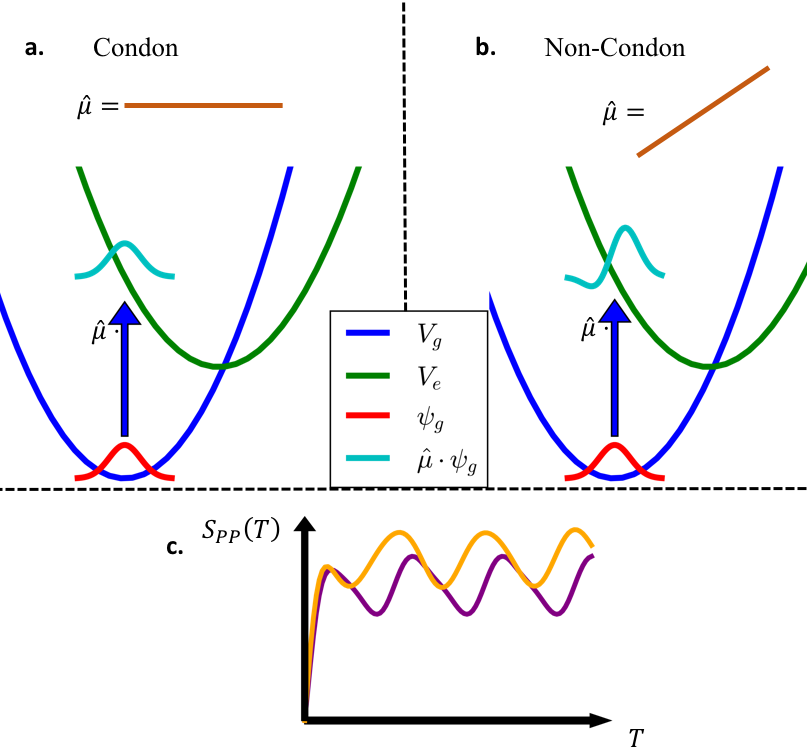
\includegraphics[width=1.0\columnwidth]{excitation_figure.png}
   \caption{In the case where there is no transition dipole variation, when the transition dipole operator is applied (with an impulsive pulse), the ground state wavepacket's shape is perfectly replicated as seen in a.  If, however, we introduce a linear variation, the wavepacket's shape is distorted as we see in b.  This manifests as a demonstrable difference in the pump probe signal as seen in c.  What is not clear is how the the signal changes as the pulse width changes for different transition dipole slopes, so we set out to investigate and see if this change keeps the protocol for electronic coherence detection proposed in ~\cite{witness,allanWitness} from working properly.  }
	\label{fig:physicalIllustration}
\end{figure}


\section{Results and Discussion}

We now have a variety of knobs to turn, in order to investigate the effect of transition dipole variation on the proposed experimental protocol.  Most importantly we have the dipole slope $\kappa/\lambda$, then the vibrational potential terms:  $\omega_{\gamma}$, $\omega_{\epsilon}$, and $\delta x$.



\begin{figure}
   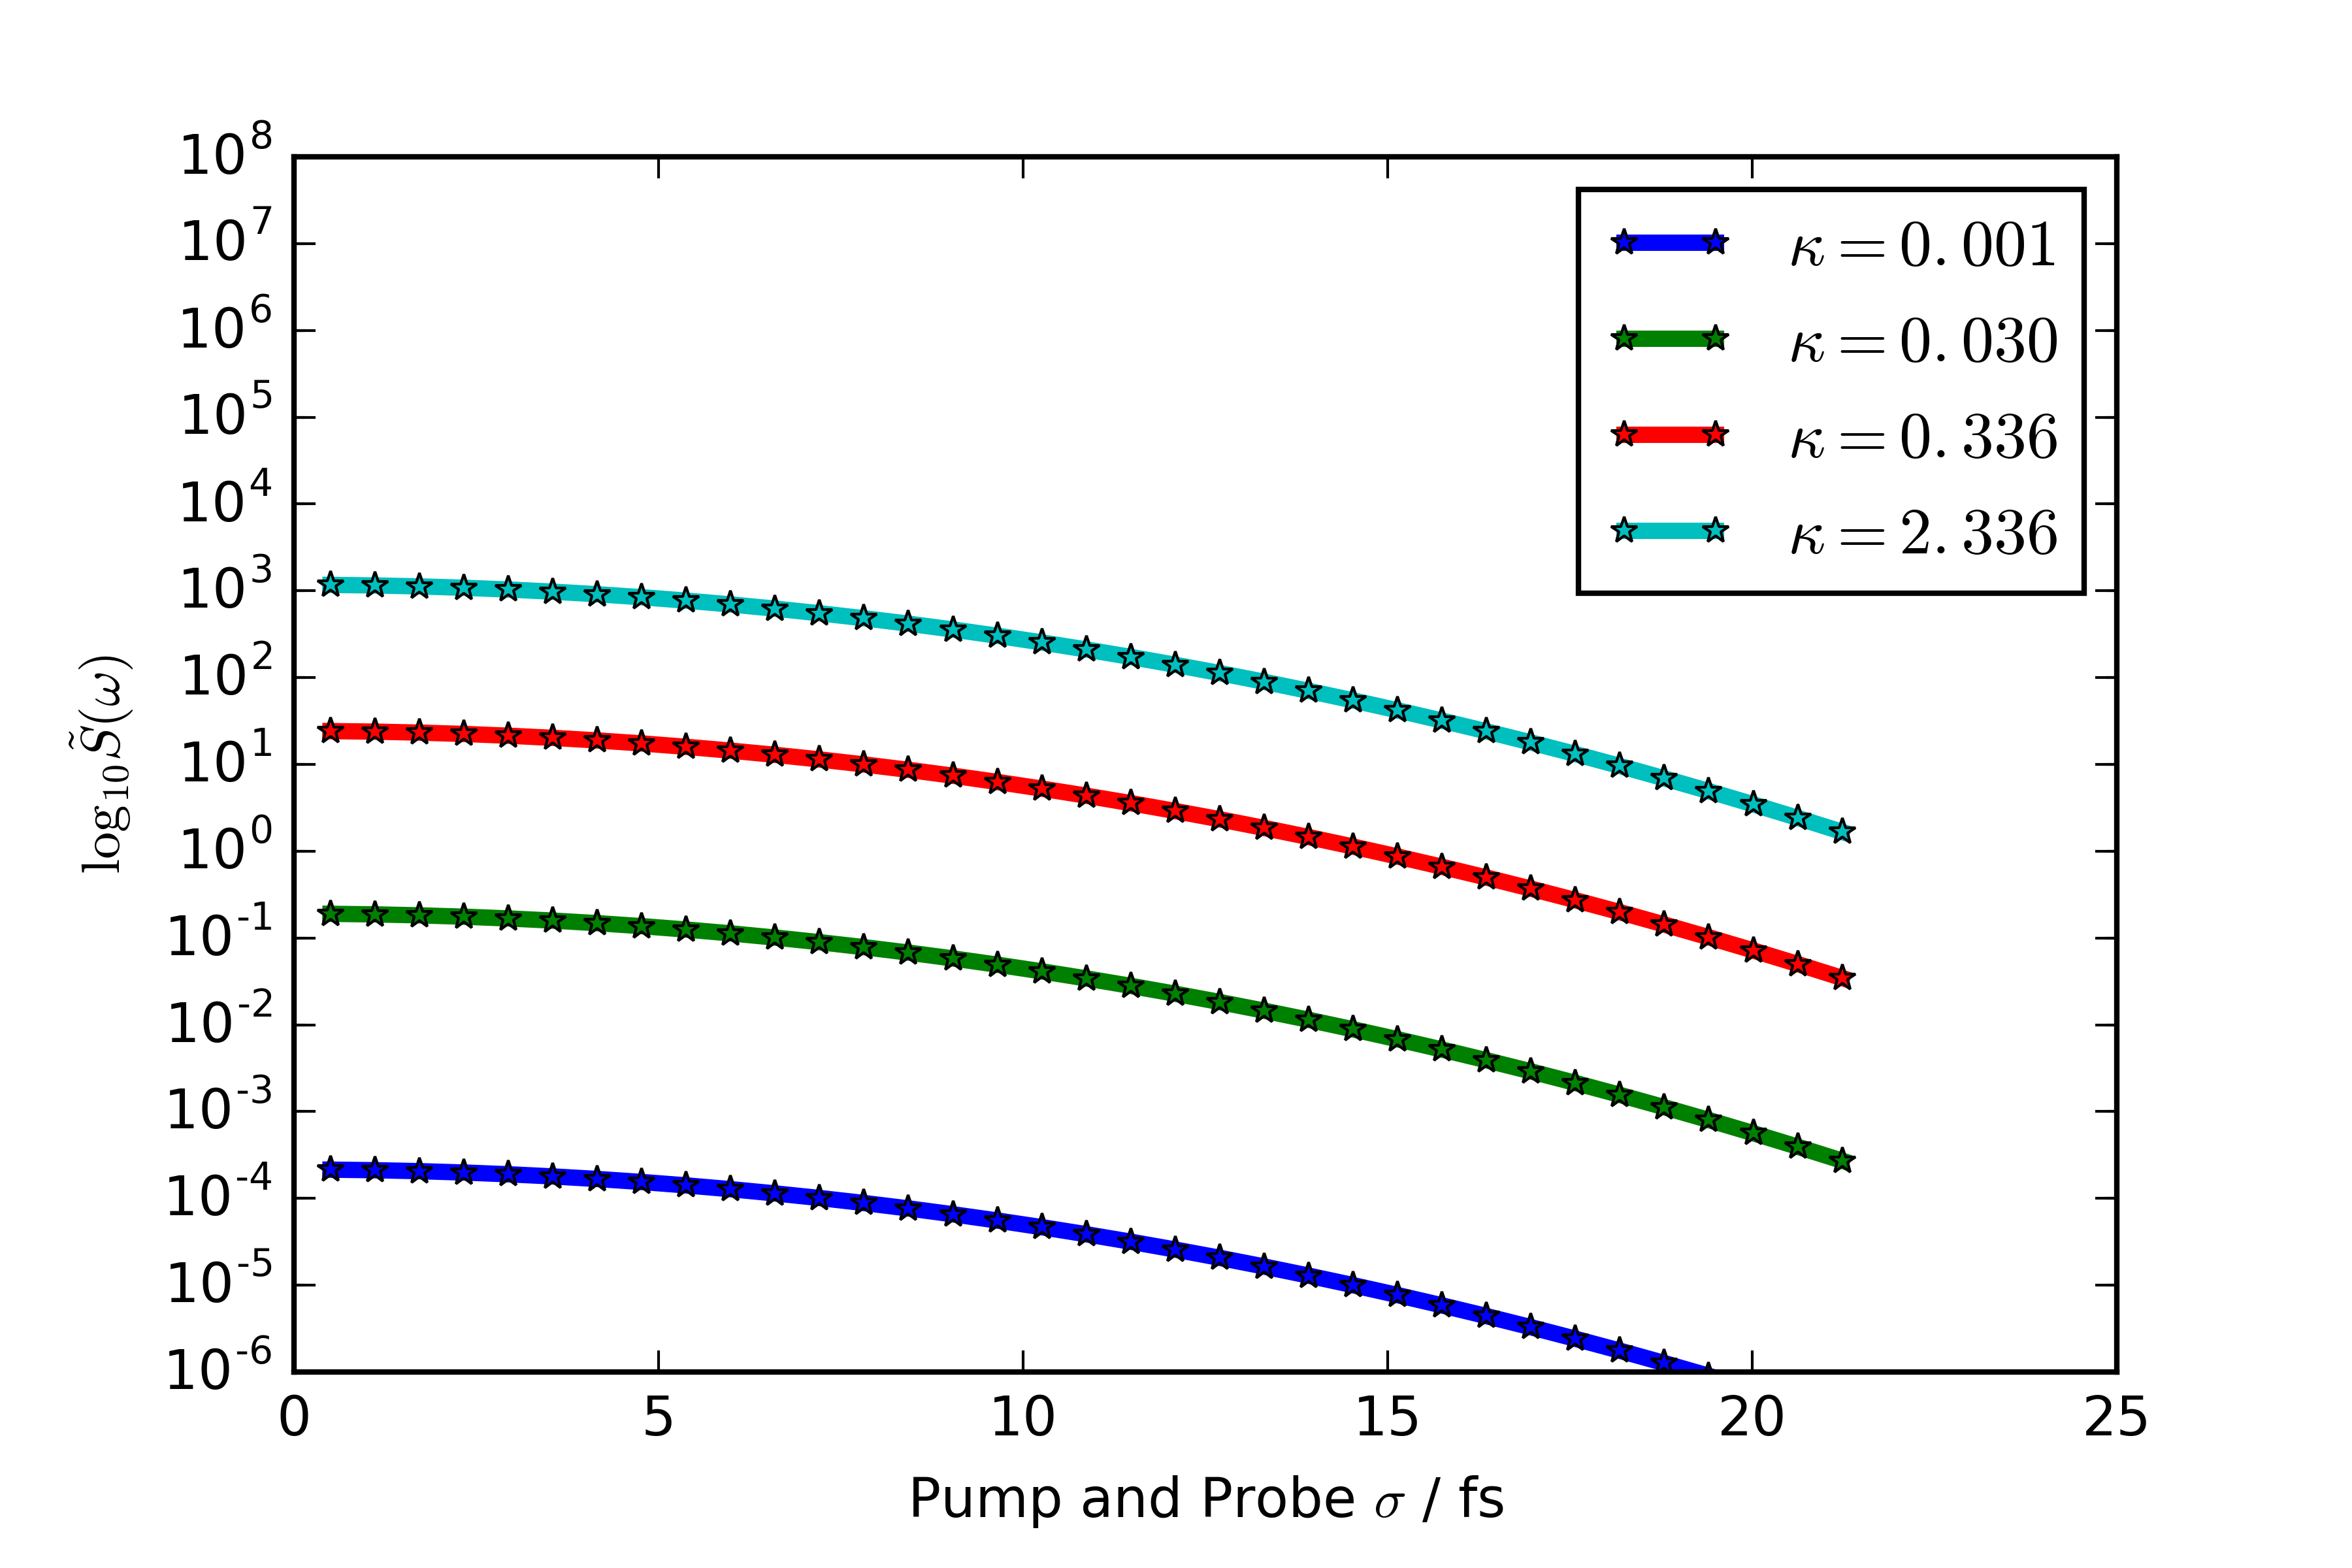
\includegraphics[width=1.0\columnwidth]{S0_samefrequency_kappa_comparison.png}
   \caption{$\tilde{S}_{PP} ( \omega)$ for a system with no vibrational displacement and $\omega_{\gamma} = \omega_{\epsilon} = \omega = $ 640 cm$^{-1}$, for various values of $\kappa$.  The y-axis is log scaled because of the signal's fourth-order dependence on $\mu(x)$; small differences in $\kappa$ make very large differences in signal.  In all of these systems, an experimenter using the proposed protocol would conclude that an electronic coherence exists in the system when there's not even a vibrational coherence in the ground state, absent a non-constant transition dipole.}
	\label{fig:tunedZero}
\end{figure}



To start with we imagine a system with a Huang-Rhys parameter of zero  ($S=0.0$) with $\omega_{\gamma} = \omega_{\epsilon}= 640 \text{cm}^{-1}$.  Because there is no difference in the vibrational manifold structure between ground and excited state, there should be no vibrational coherence; only the 0th state is important in both wells.  So this should definitely not have any oscillations at any pulse width when we induce a nonzero $\kappa$ cut as can be seen in figure \ref{fig:tunedZero}, they not only oscillate but have growing oscillations as the pulse width decreases.  That would mean that according to the protocol of ~\cite{witness,allanWitness}, one would diagnose an electronic coherence in this system, when there's not even really a vibrational coherence in the sense that we think of one.

A system like the one from above has little use outside of theory, because its highly improbable for a system to not change its vibrational structure at all when its electronic structure undergoes a shift.  So we continue to a system where $S=0.005$ which is close to what photosynthetic Huang-Rhys factors are~\cite{typicalHRFforPhotosynthesis}.


\begin{figure}
   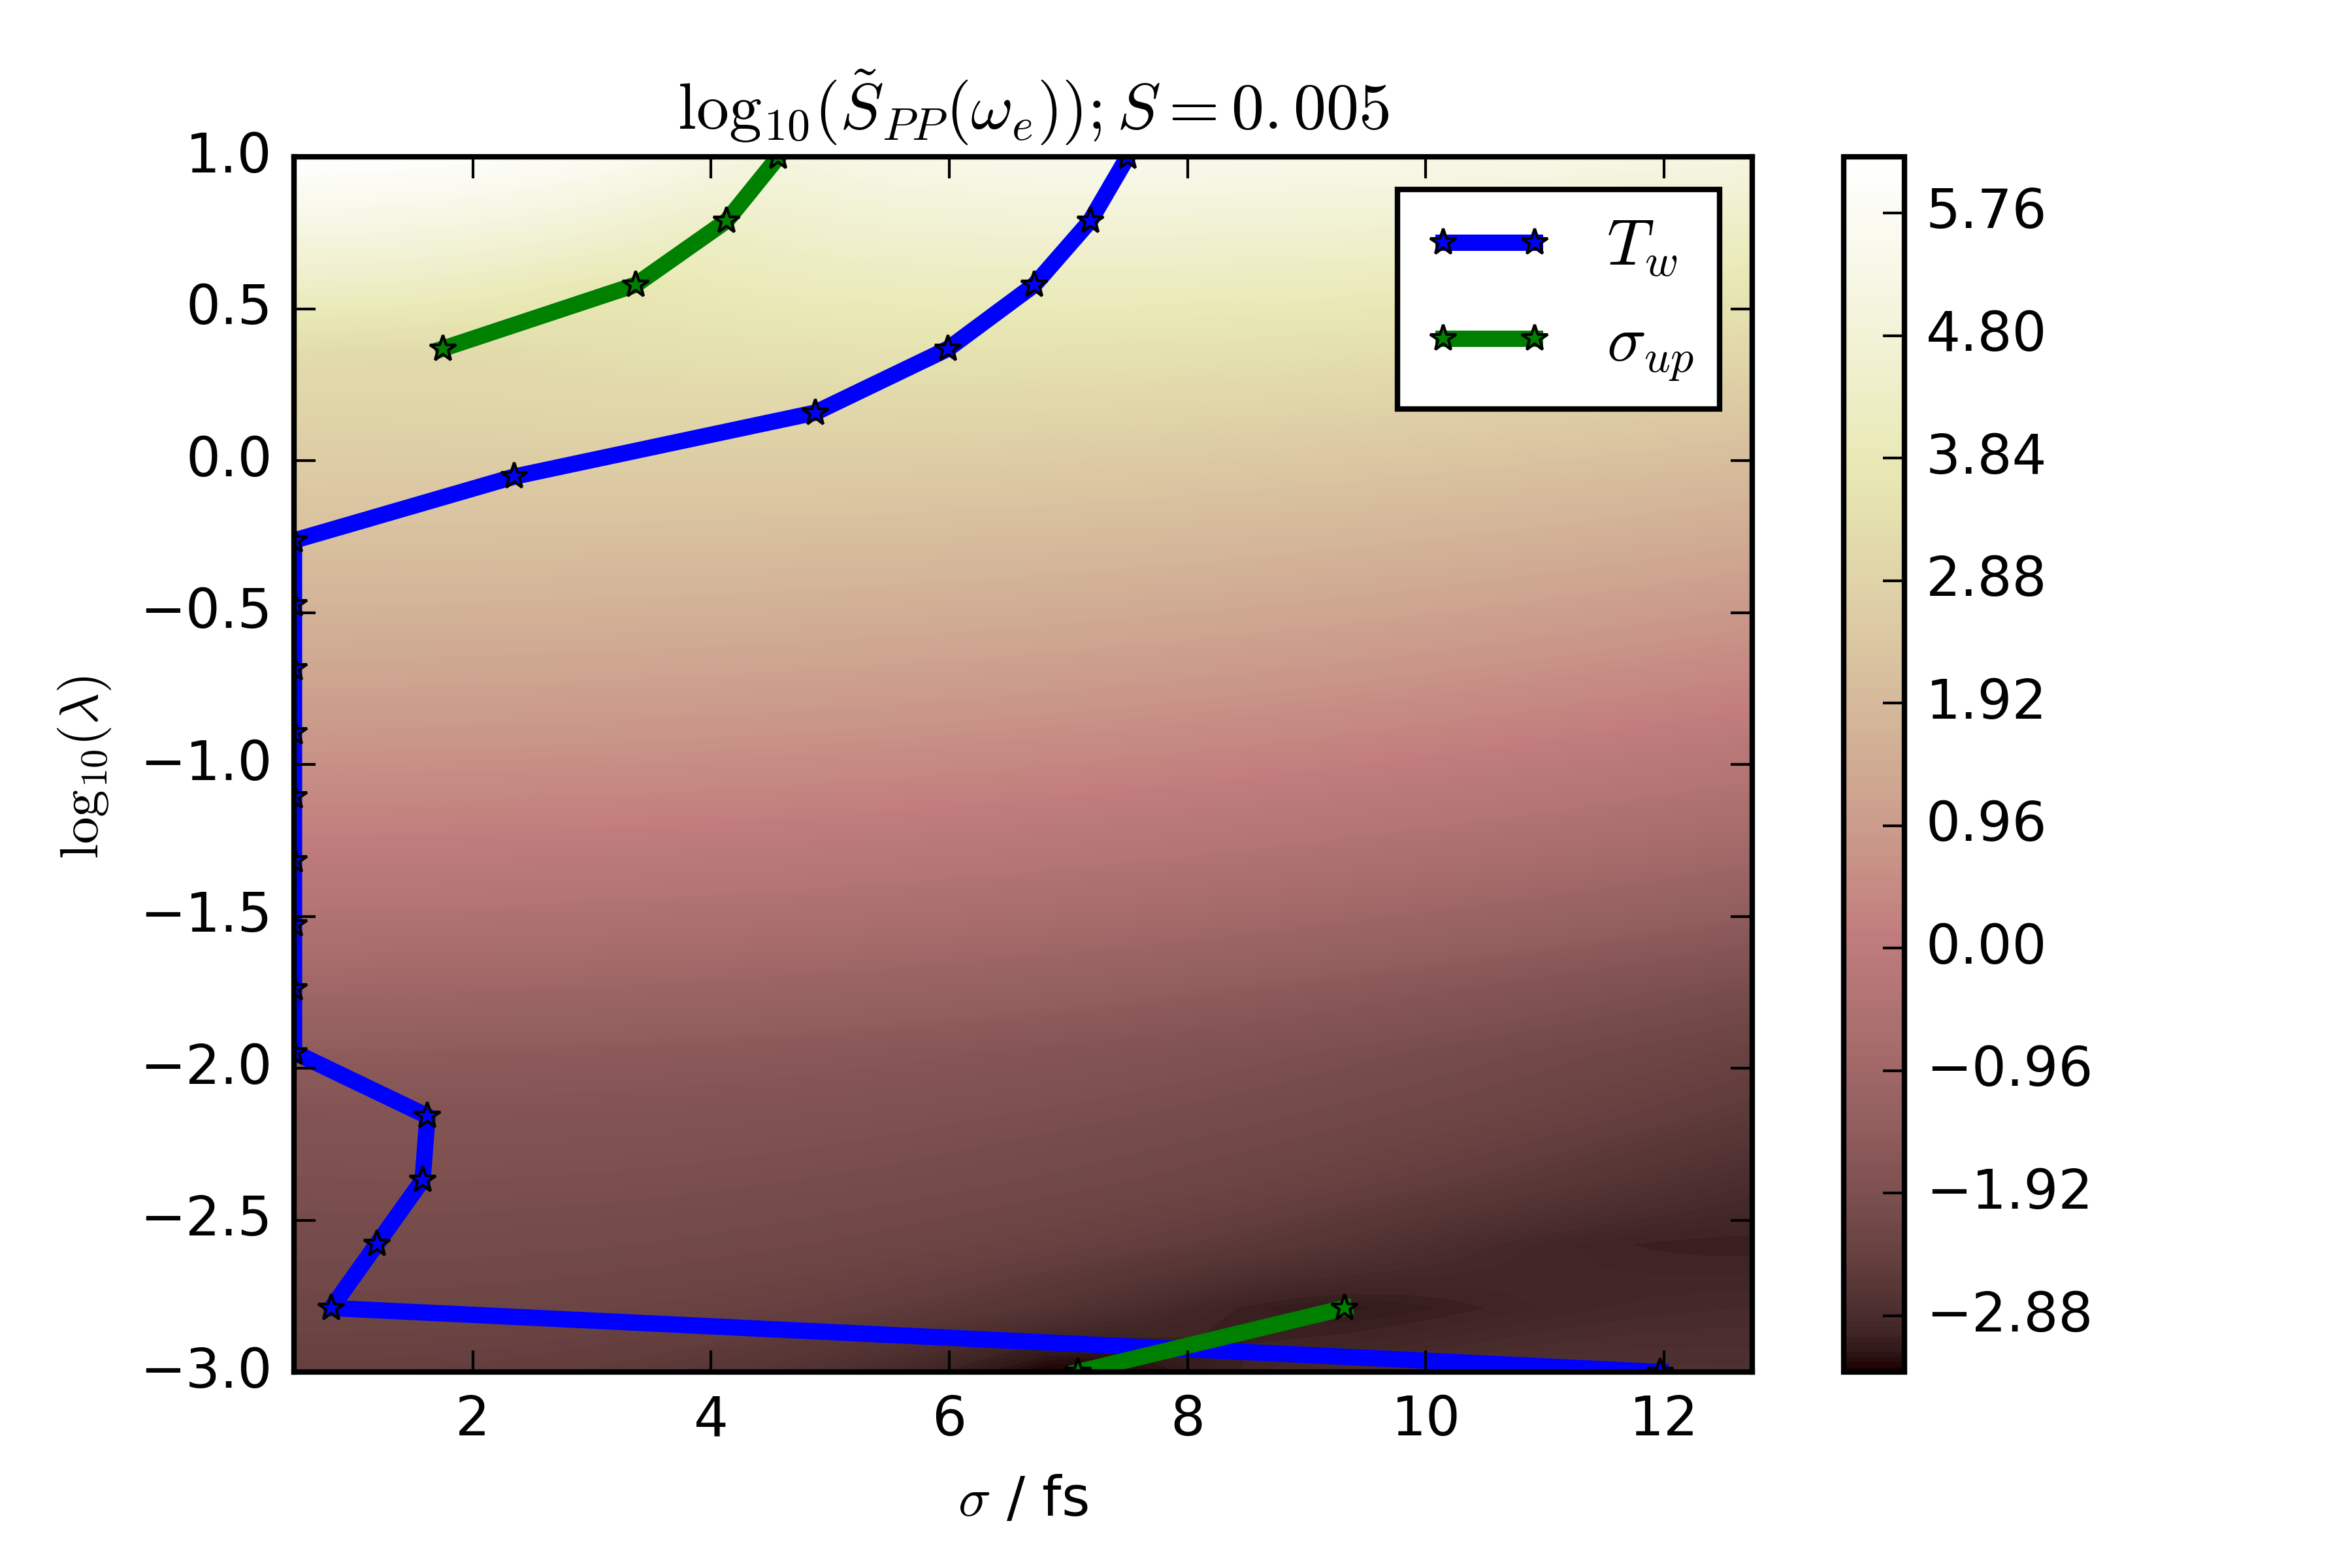
\includegraphics[width=1.0\columnwidth]{S_0p005_contour.png}
   \caption{$\tilde{S}_{PP} ( \omega_e)$ as a function of $\lambda$ and the pulse width $\sigma$ in a system where S=0.005, $\omega_e = .9 \omega_g$. and $\omega_g = 640 \text{cm}^{-1}$. $T_w$ is the same as defined in reference \cite{allanWitness}: the peak of the signal before it goes down again.   Some traces in $\lambda$ have local minima as well when the signal goes up and we plot those as $\sigma_{up}$.  In the case where the signal just goes up as the pulse width goes down, then $T_w$ is set as $\sigma=0$}
	\label{fig:s_0p005}
\end{figure}

As can be seen in Figure \ref{fig:s_0p005}, there is basically nowhere that the protocol works and, worryingly, in the region of $\lambda = .1$, the signal monotonically goes up, just like the $S=0.0$ case.  While the signal does go down from its peak for some values of $\lambda$, this is before experimental noise considerations are taken into account.

We next look at a larger value of the Huang-Rhys parameter: $S=.2$.  We then plot the values of the signal oscillations again as a function of lambda and the result can be seen in Figure \ref{fig:s_0p2}.

\begin{figure}
   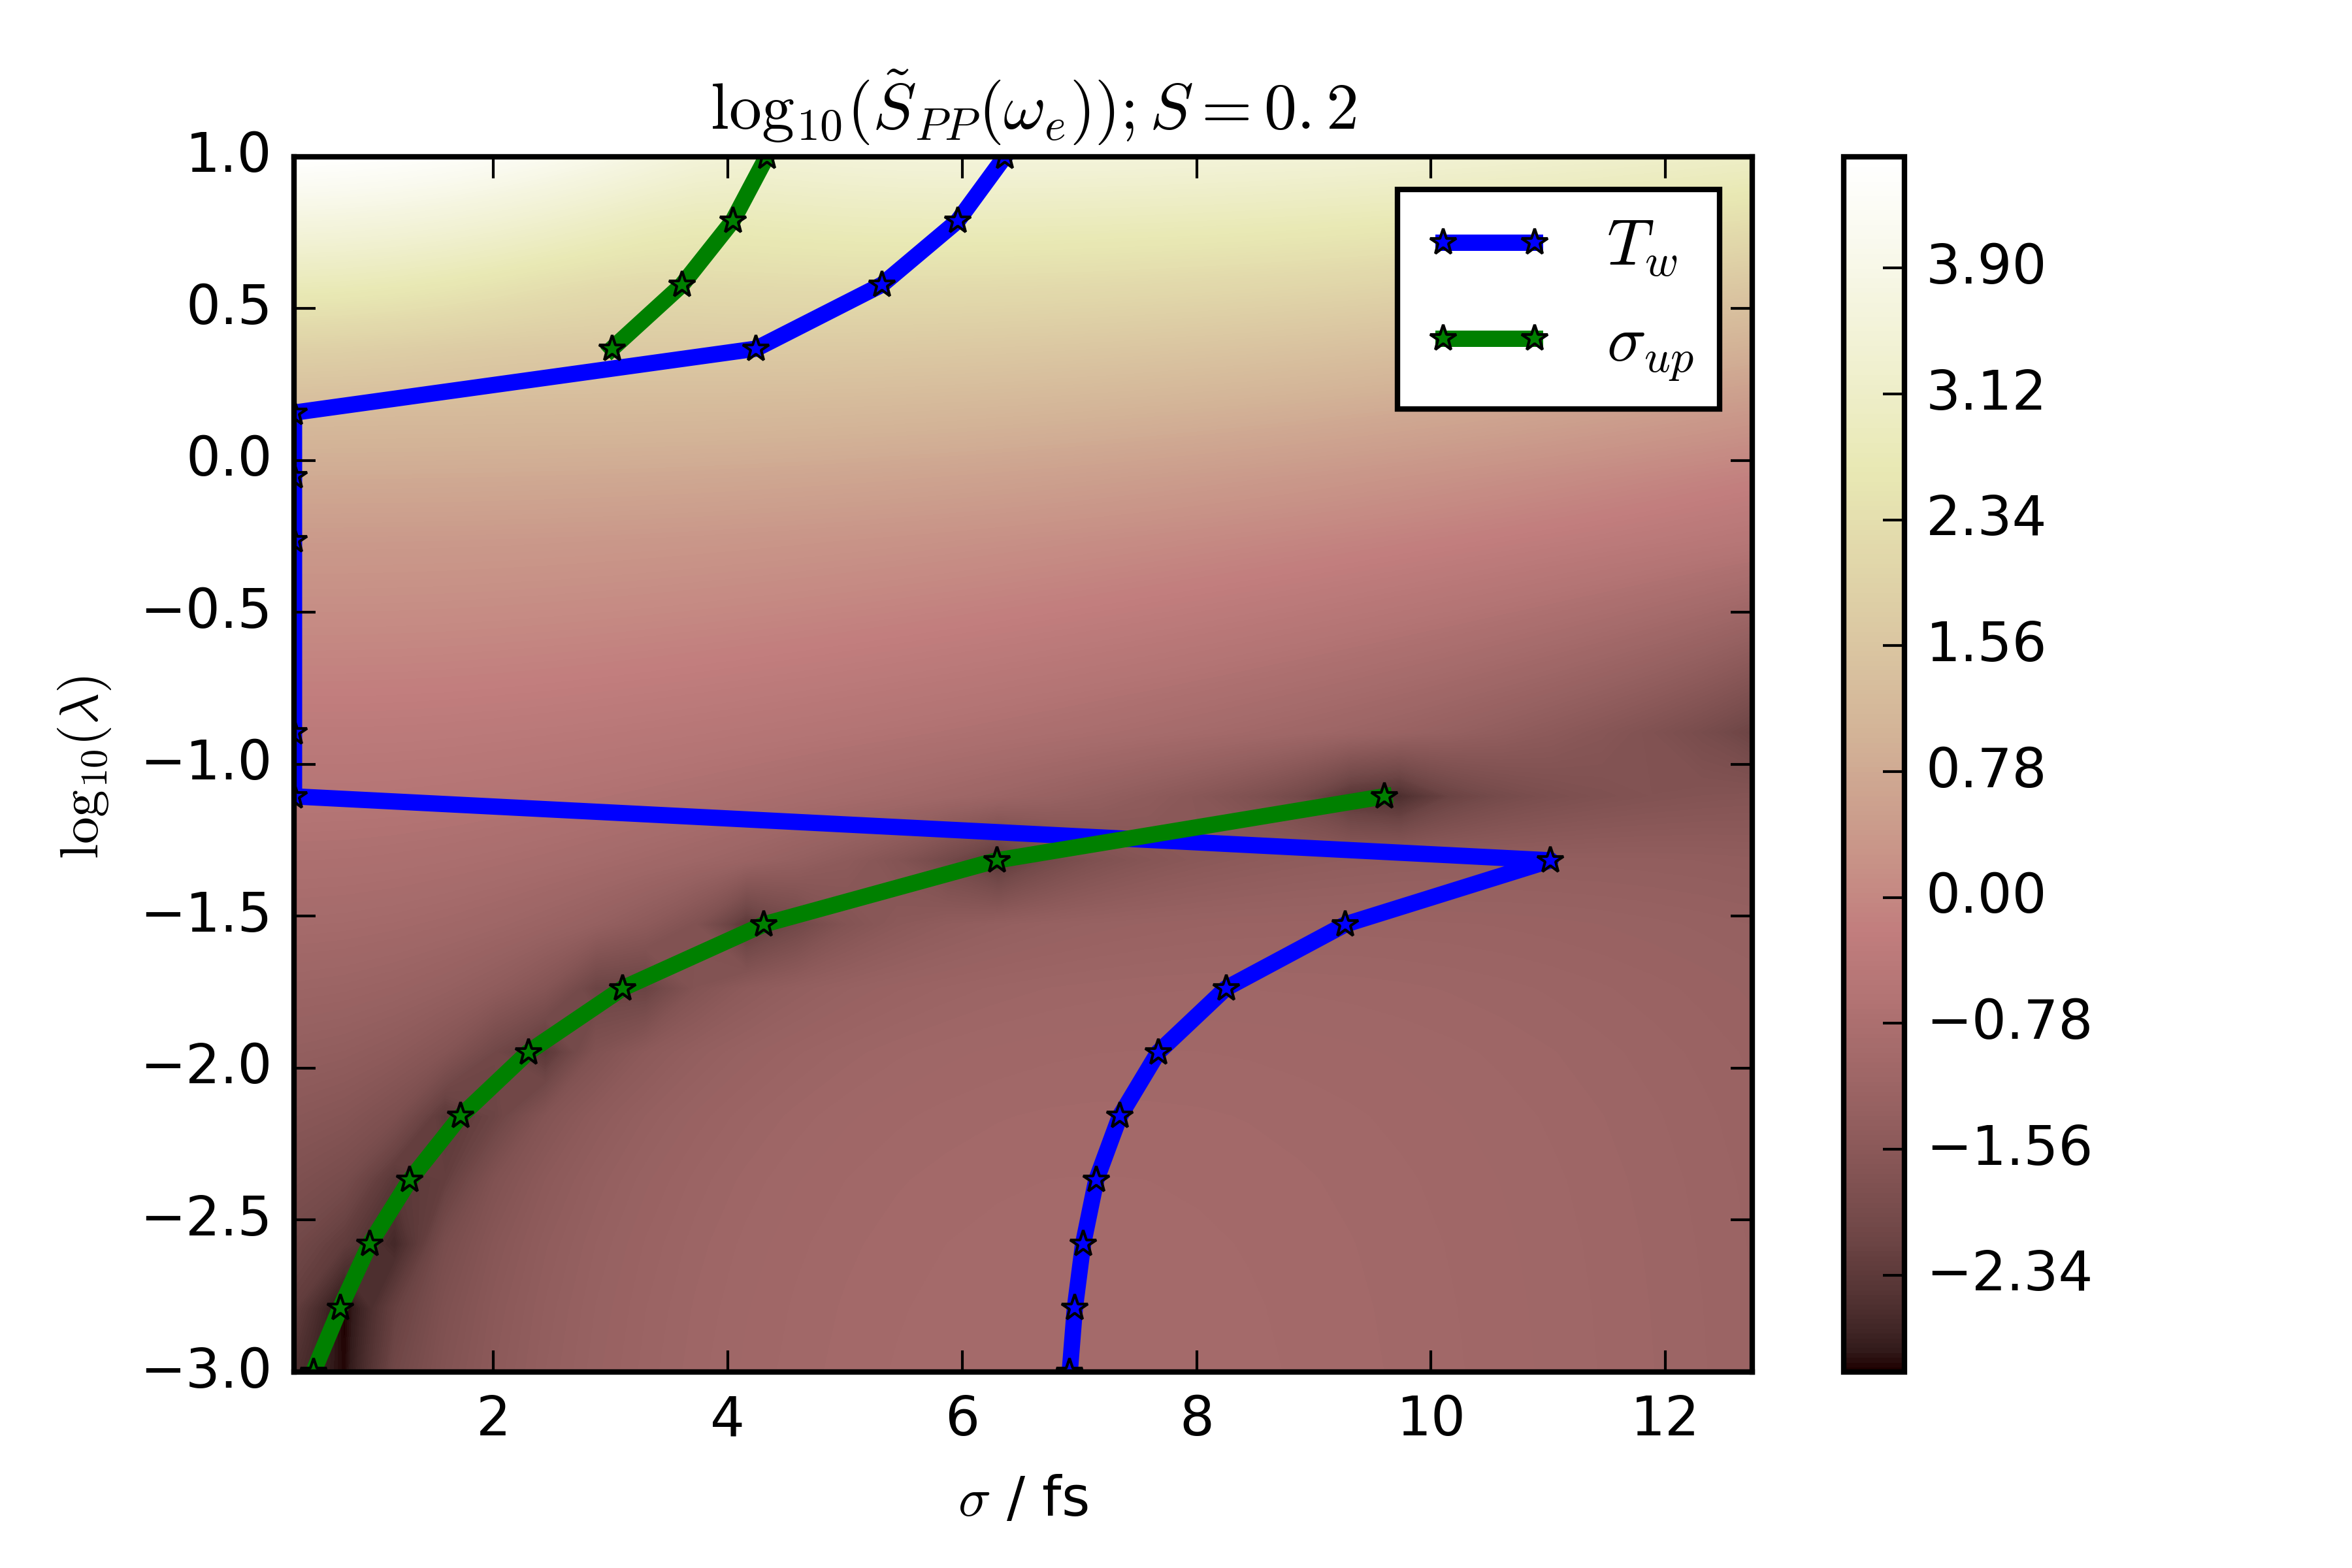
\includegraphics[width=1.0\columnwidth]{S_0p2_contour.png}
   \caption{$\tilde{S}_{PP} ( \omega_e)$ as a function of $\lambda$ and the pulse width $\sigma$ in a system where S=0.2, $\omega_e = .9 \omega_g$. and $\omega_g = 640 \text{cm}^{-1}$. }
	\label{fig:s_0p2}
\end{figure}

This seems to suggest that for larger values of $S$, there are fewer false positives in the proposed protocol, but still indicates that there are many regions where false positives exist.


As to the origins of the observed dips in the signal seen in Figures \ref{fig:s_0p005} and \label{fig:s_0p2},in figure \ref{fig:addedSignals}, when the nonzero $\kappa$ is turned off, we get a decreasing oscillatory signal approaching zero as the laser pulse width approaches zero just as predicted by ~\cite{allanWitness}.  If, however, we turn on the nonzero $\kappa$, we see the while there is a dip at a certain point in the signal, it increases as the pulse width approaches zero.  Indeed, even if we set $S=0.0$, and thus have a system that should have almost no oscillations, there is still an increasing oscillation signal.  The shape of these three curves suggests that there is an interference interplay between the tendency of a vibrational coherence to go down as the pulse width approaches zero and the tendency of an oscillation induced by a linear transition dipole variation to increase as the pulse width gets toward zero.

\begin{figure}
   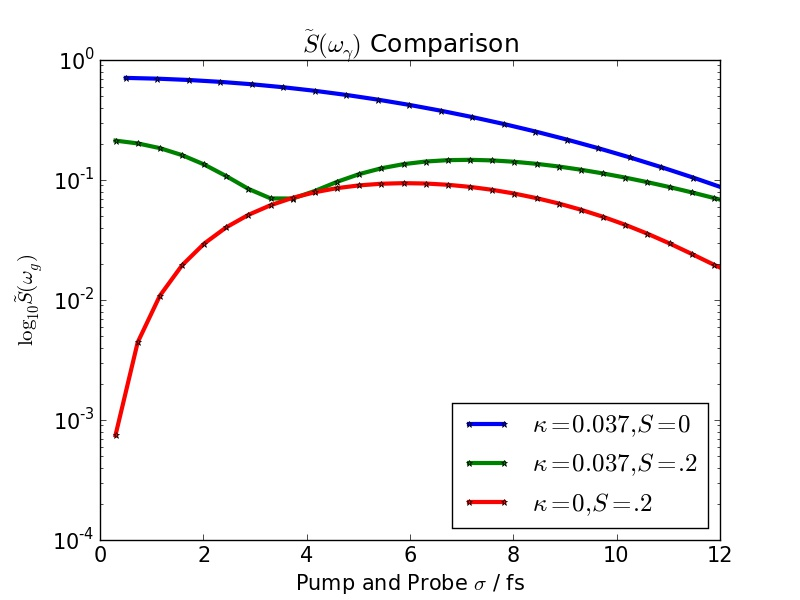
\includegraphics[width=1.0\columnwidth]{comparison_omega_g.jpg}
   \caption{$\tilde{S}_{PP} ( \omega_{\gamma})$ Here we have plotted the ground state oscillations for 3 systems: $\kappa=.037, S=0$; $\kappa=.037, S=0.2$; and $\kappa=0.0, S=0.2$.  This shows roughly that the effects of a non-Condon monomer without vibrational displacement add together with the effects of a Condon monomer to get the result for a non-Condon monomer with a vibrational displacement}
	\label{fig:addedSignals}
\end{figure}




\section{Conclusion}

Given all we have seen at this point, we must caution against using the protocol suggested by ~\cite{witness} and refined by ~\cite{allanWitness} to diagnose the existence or non-existence of long-lived electronic coherences in any kind of system, without first knowing about the extent to which the transition dipole is non-constant with respect to the relevant nuclear coordinates.  Future work may be able to salvage this protocol or a similar protocol, but without a good tool to determine whether a system has a sizeable variation in its transition dipole, there is no way to make sense of the pulse-width-dependent increasing or decreasing pump probe signal oscillations without ambiguity.

% [Doran's suggestion:  Possibly add a discussion about how non-Condon effects could alter the interpretation of an existing experiment?  After looking at every paper citing Joel and Allan's witness, nothing jumps out at me as a good example of how non Condon moments can effect an observable.  Any technique which only considers a certain number of vibrational states is in danger of considering too few in any non Condon case.]



\section{Acknowledgments}
We acknowledge the support from the Center for Excitonics, an Energy Frontier Research Center funded by the U.S. Department of Energy under award DE-SC0001088 (Solar energy conversion process).  The authors also wish to thank Doran Bennet for his useful commentary on this manuscript.  We want to further acknowledge the previous work of Joel Yuen-Zhou and Allan Johnson, upon which we could not have continued without.



\section{Supplemental Materials}
We have $\lambda$ scans for $S=.4$ and $S=1.0$ as well.  Figure \ref{fig:s_1p0} and \ref{fig:s_0p4} paint a picture suggesting that the higher the Huang-Rhys parameter, the more valid the article proposed in ~\cite{allanWitness} and ~\cite{witness} will work.  The larger values of $S$ to indeed have fewer regions of false-positives.
\begin{figure}
   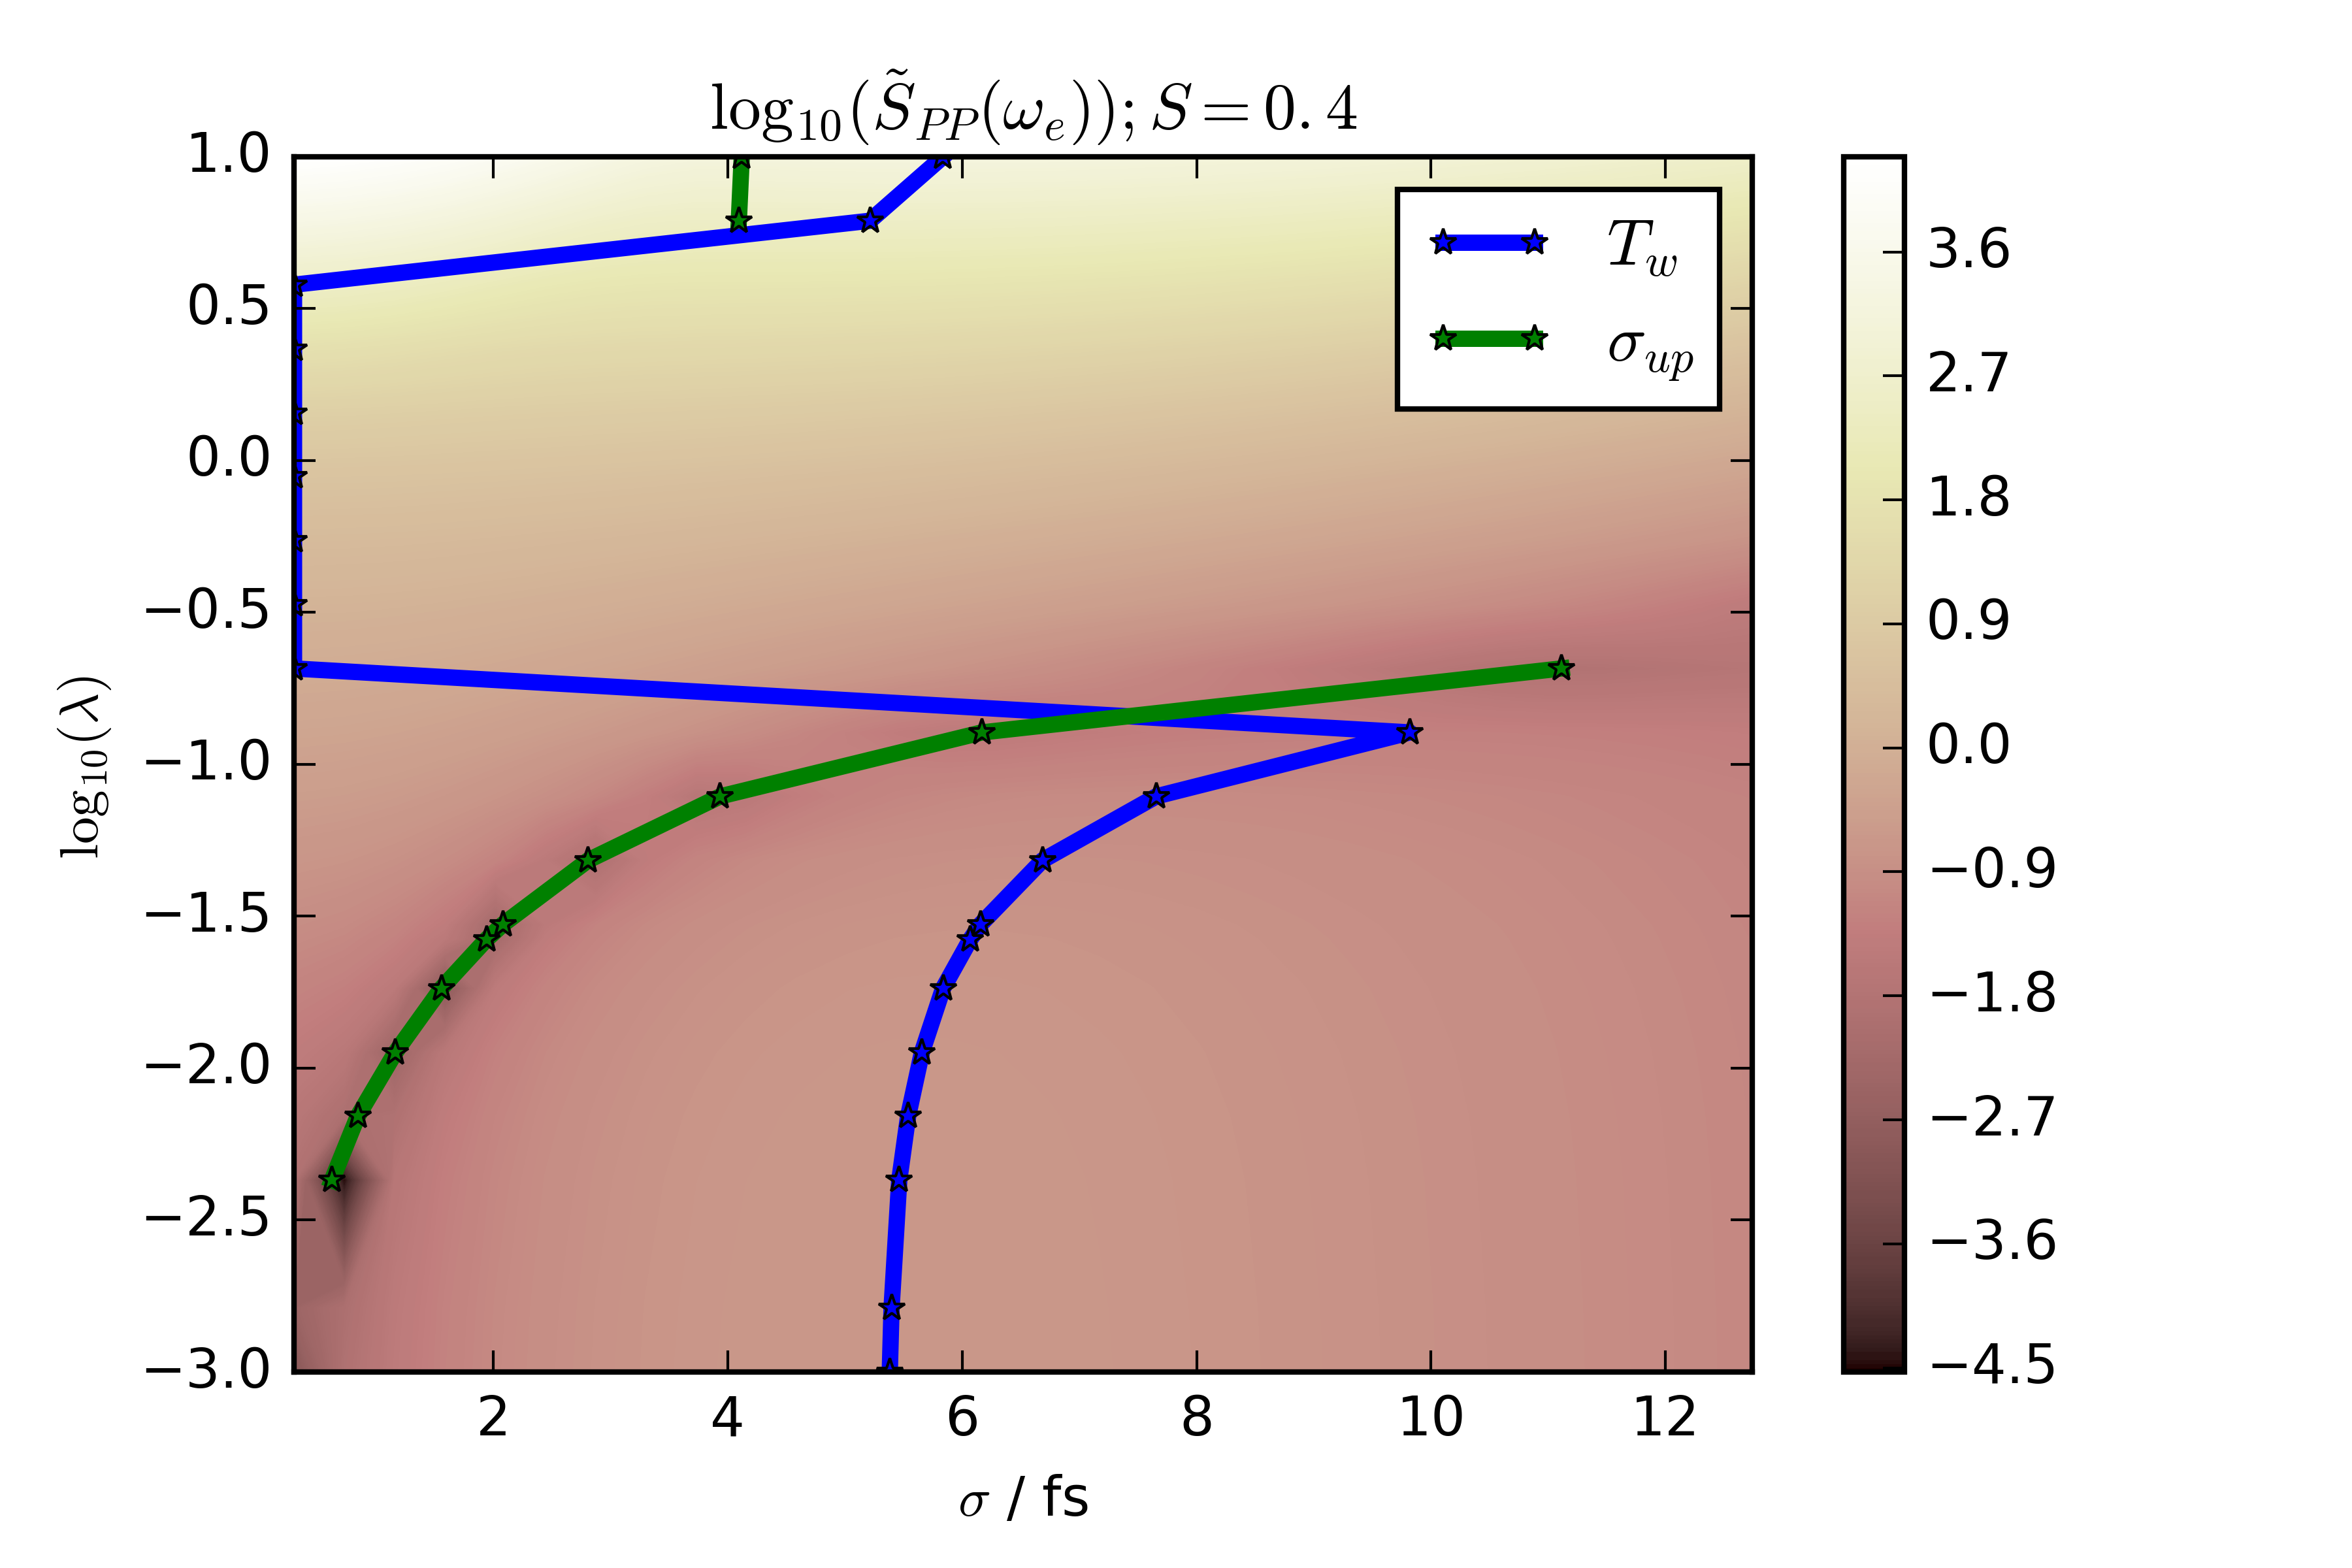
\includegraphics[width=1.0\columnwidth]{S_0p4_contour.png}
   \caption{$\tilde{S}_{PP} ( \omega_e)$ as a function of $\lambda$ and the pulse width $\sigma$ in a system where S=0.4, $\omega_e = .9 \omega_g$. and $\omega_g = 640 \text{cm}^{-1}$.}
	\label{fig:s_0p4}
\end{figure}

\begin{figure}
   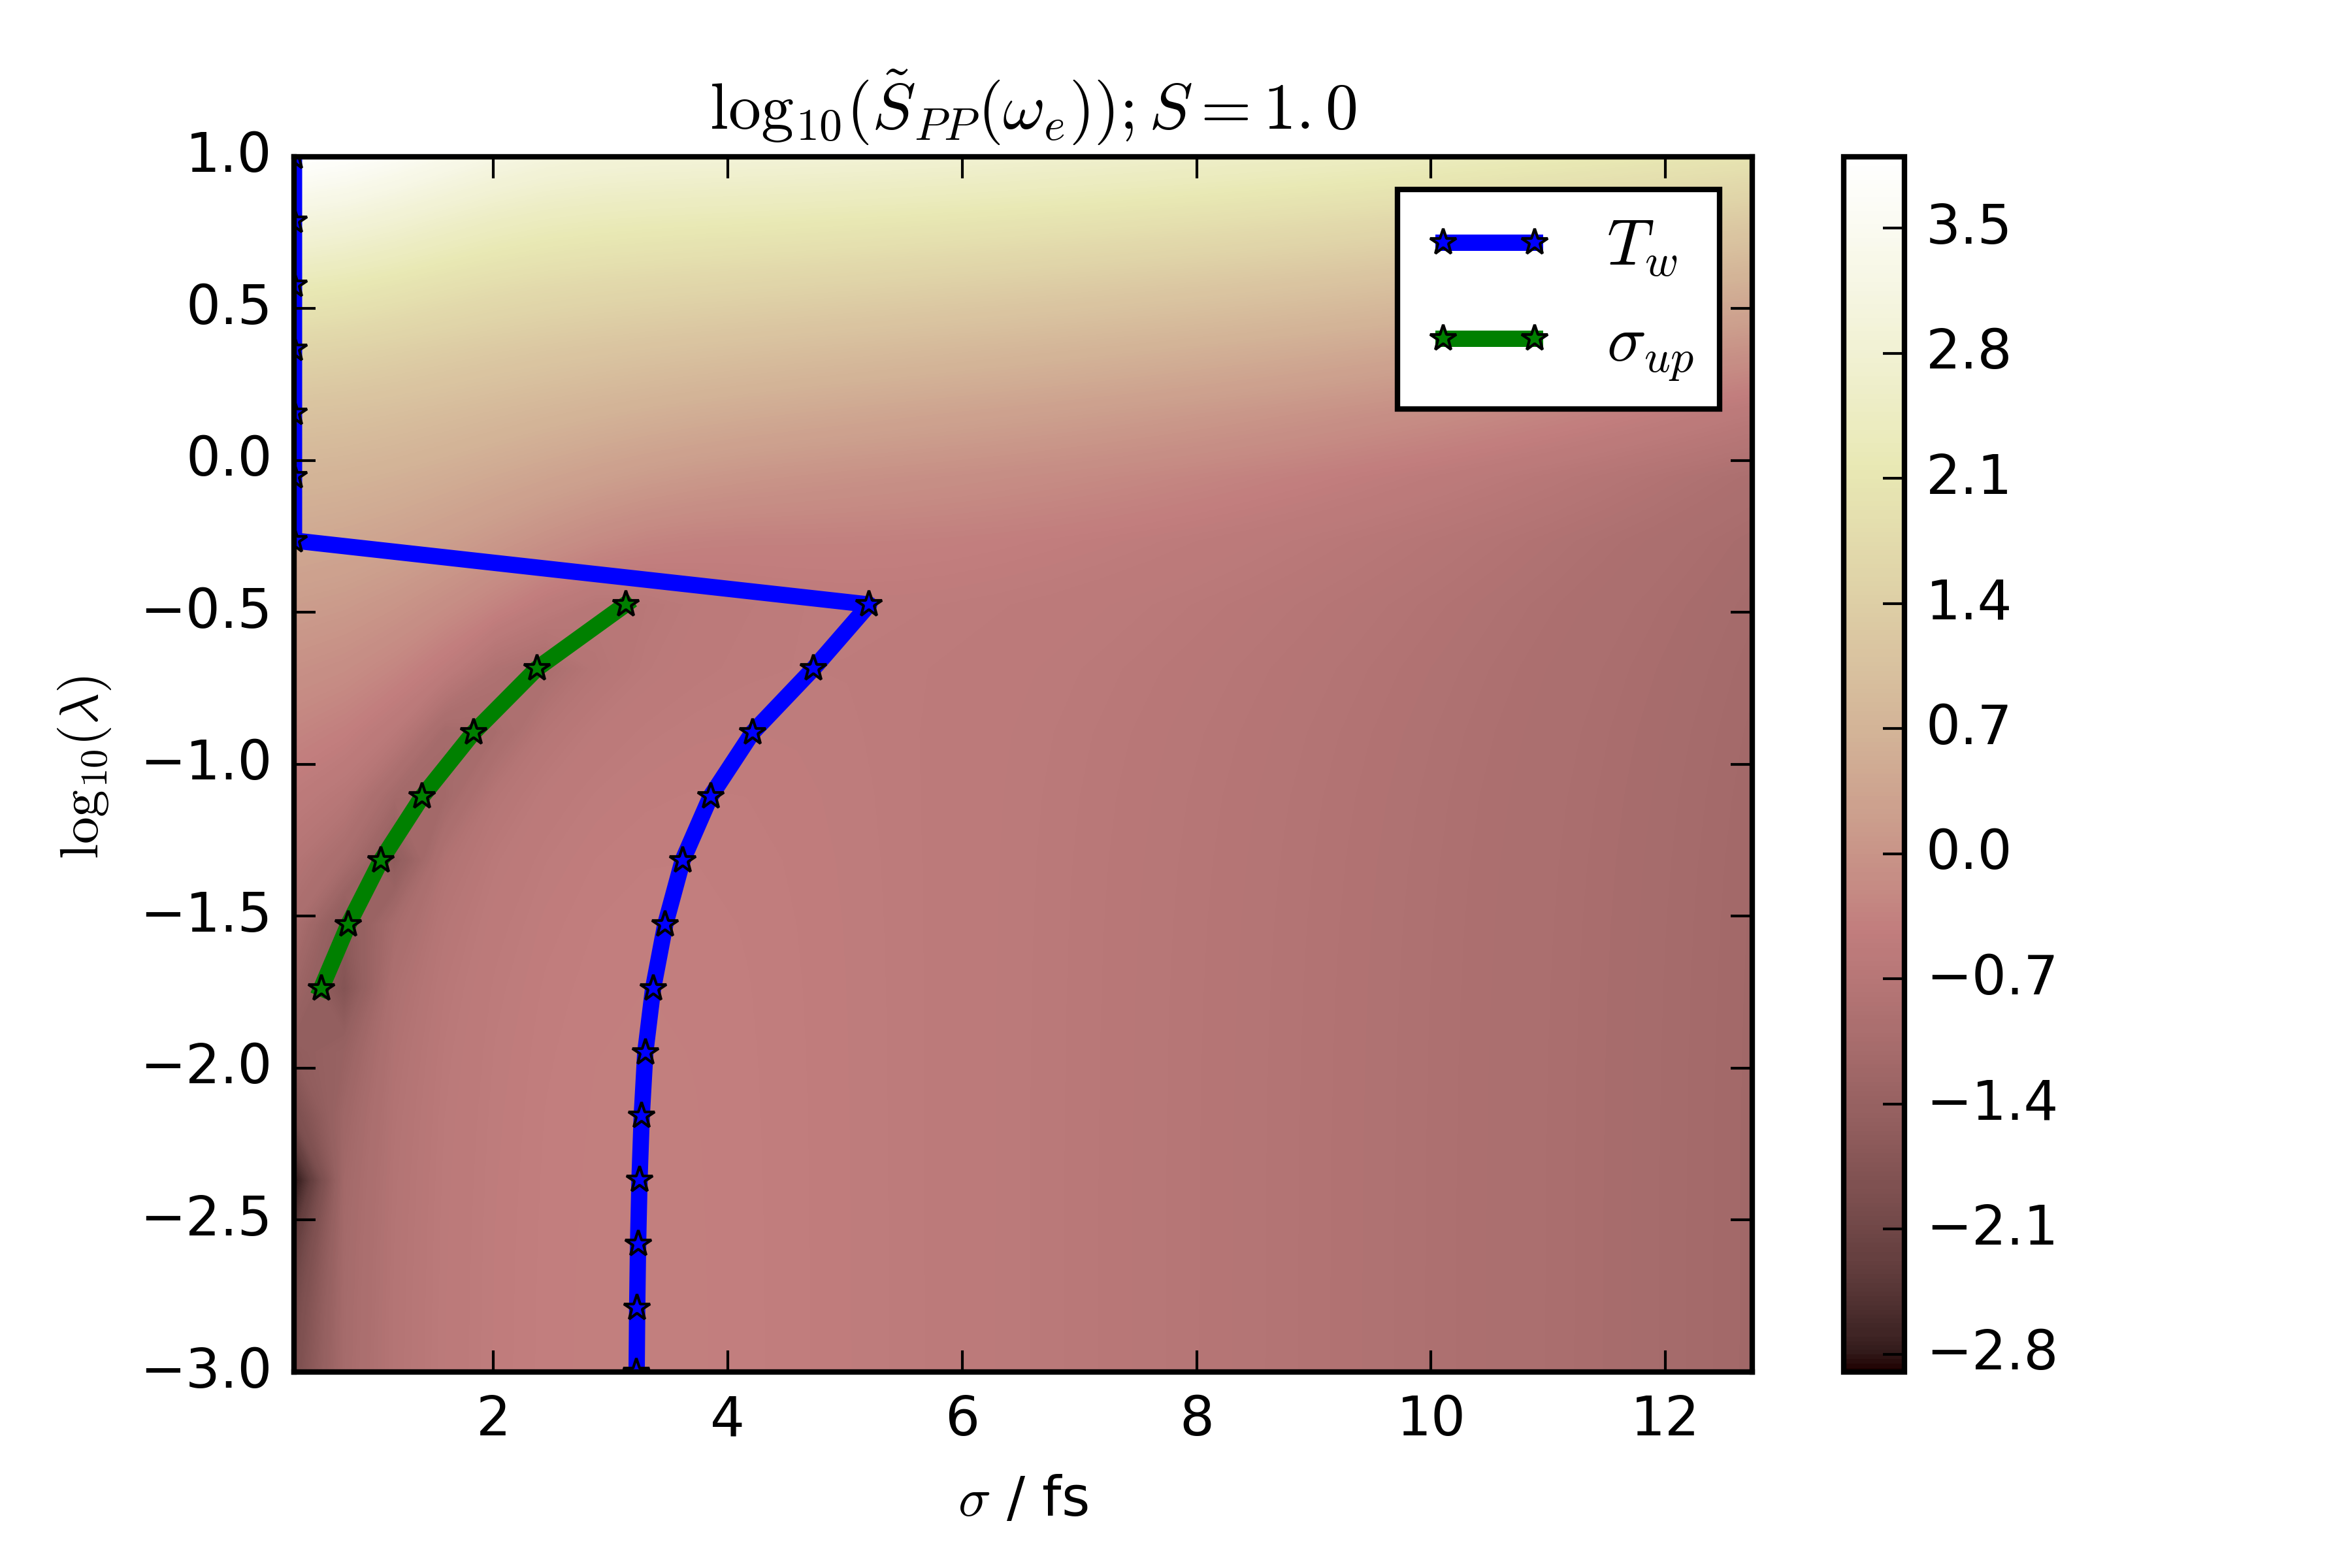
\includegraphics[width=1.0\columnwidth]{S_1p0_contour.png}
   \caption{$\tilde{S}_{PP} ( \omega_e)$ as a function of $\lambda$ and the pulse width $\sigma$ in a system where S=1.0, $\omega_e = .9 \omega_g$. and $\omega_g = 640 \text{cm}^{-1}$. }
	\label{fig:s_1p0}
\end{figure}
We caution, however, as we suspect that the existence of an upturn in our data  is also a function of the minimum pulse width as a ratio of the vibrational frequency of the system.  For all of the simulations in this paper, $\sigma_{\min} \omega_{\gamma} \approx 0.04 $, so for vibrational modes and experiments with regions where that figure of merit can be smaller, there are even fewer regions where there are no false positives in the proposed protocol.
